%
% introduction.tex
%
% Copyright (C) 2021 by SpaceLab.
%
% TTC 2.0 Documentation
%
% This work is licensed under the Creative Commons Attribution-ShareAlike 4.0
% International License. To view a copy of this license,
% visit http://creativecommons.org/licenses/by-sa/4.0/.
%

%
% \brief Introduction chapter.
%
% \author Gabriel Mariano Marcelino <gabriel.mm8@gmail.com>
%
% \institution Universidade Federal de Santa Catarina (UFSC)
%
% \version 0.1.0
%
% \date 2021/04/01
%

\chapter{Introduction} \label{ch:introduction}

The TTC 2.0\nomenclature{\textbf{TTC}}{\textit{Telemetry, Tracking and Command.}} is an Telemetry, Tracking and Command module designed for nanosatellites. It is one of the service modules developed for the FloripaSat-2 CubeSat Mission \cite{floripasat2}.

The module is a direct upgrade from the TTC of FloripaSat-1 \cite{ttc-fsat}, which grants a flight heritage rating. The improvements focus on providing a cleaner and more generic implementation in comparison with the previous version, more reliability in software and hardware implementations, and adaptations for the new mission requirements. All the project, source and documentation files are available freely on a GitHub repository \cite{ttc2-repo} under the GPLv3 license.

\begin{figure}[!h]
	\begin{center}
		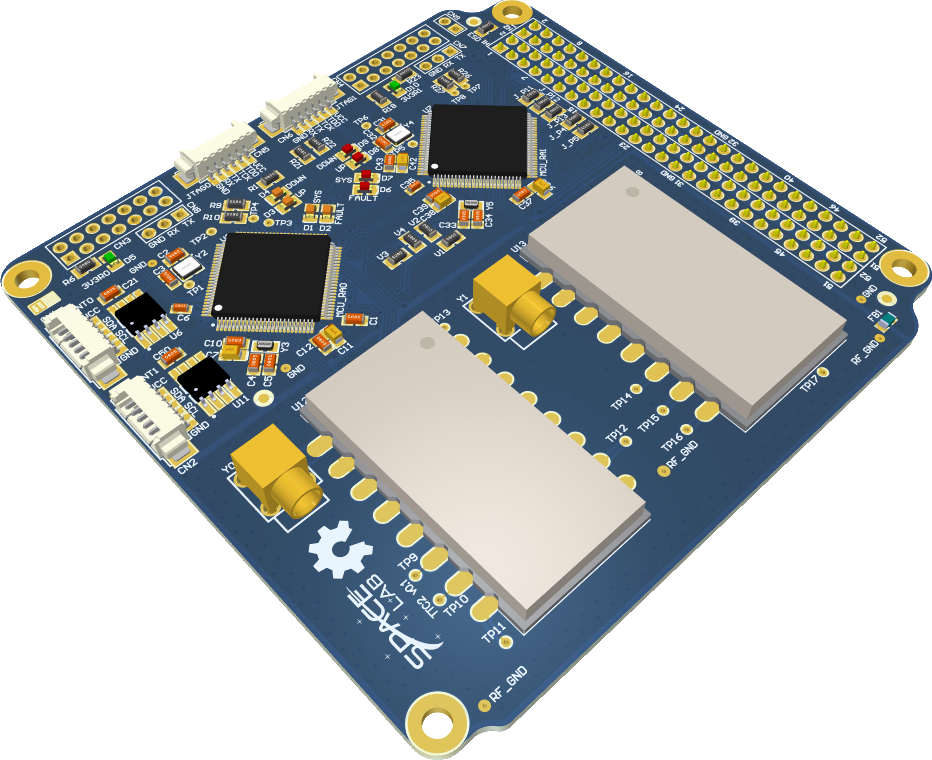
\includegraphics[width=0.65\textwidth]{figures/ttc2_pcb_3d.png}
		\caption{3D view of the TTC 2.0 PCB\nomenclature{\textbf{PCB}}{\textit{Printed Circuit Board.}}.}
		\label{fig:pcb-3d}
	\end{center}
\end{figure}
